\documentclass[handout, 11pt]{beamer}
\mode
<presentation>{\usetheme{Madrid}}
\institute[UF]{\inst{1}
University of Florida\\
Department of Finance, Insurance, and Real Estate}
\usepackage{adjustbox}
\usepackage{tikz}
\usepackage{minted}
\definecolor{darkgreen}{RGB}{31,156,17}
\usepackage{booktabs}
\usepackage{xcolor}
\setbeamertemplate{headline}{\begin{beamercolorbox}[ht=2.25ex, dp=3.75ex]{section in head/foot}
\insertnavigation{\paperwidth}
\end{beamercolorbox}}
\AtBeginSection{\begin{frame}
\frametitle{Table of Contents}
\tableofcontents[currentsection]
\end{frame}}
\begin{document}
\title[Python Basics]{Going Beyond an Initial Python Script}
\subtitle{How to Structure Python Code and Common Operations}
\author[DeRobertis]{Nick DeRobertis\inst{1}}
\date{\today}
\begin{frame}
\titlepage
\label{title-frame}
\end{frame}
\begin{section}[Intro]{Introduction}
\begin{frame}
\frametitle{An Organized Structure of an Advanced Python Model}
\begin{columns}
\begin{column}{0.5\textwidth}
\vbox to 0.8\textheight{\begin{itemize}
\item Now we are going to build our first complex Python model
\vfill
\item We will also learn a bit more Python before we can get there
\vfill
\item Just as we did in Excel, we need to add structure to make the model navigatable
\vfill
\item Logic should be organized in functions and be documented
\end{itemize}}
\end{column}
\begin{column}{0.5\textwidth}
\vbox to 0.8\textheight{\centering
\vfill

\includegraphics[height=1.0\textheight, keepaspectratio, width=0.9\textwidth]{Sources/python-logo.png}
\vfill
\vfill}
\end{column}
\end{columns}
\end{frame}
\begin{frame}
\frametitle{The Structure of a Complex Model}
\begin{center}
\begin{adjustbox}{width=0.9\textwidth, height=0.8\textheight, keepaspectratio}
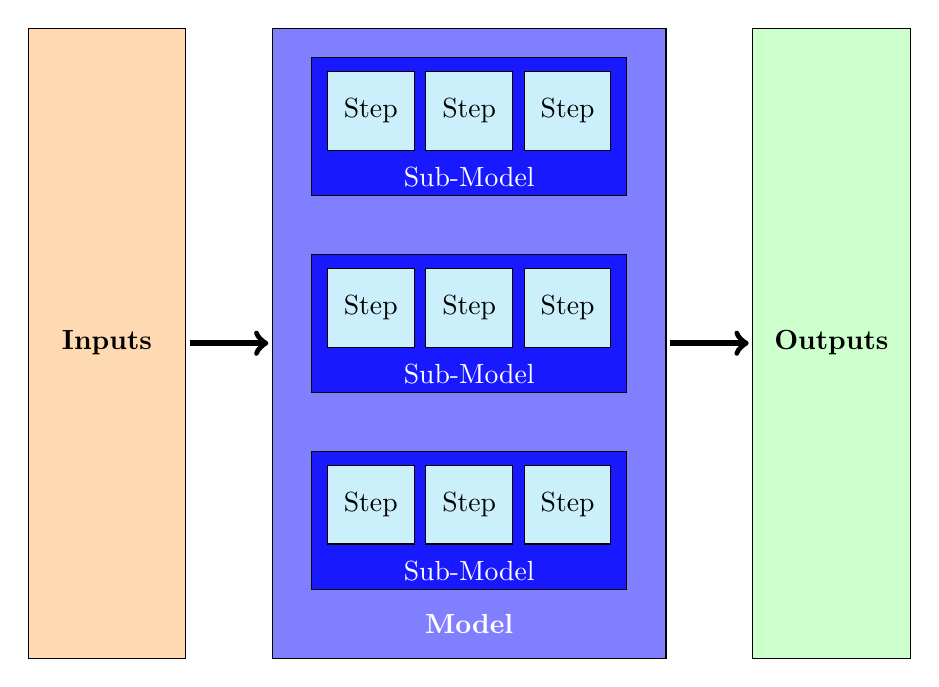
\begin{tikzpicture}
\node [fill=orange!30, minimum width=2cm, minimum height=8cm, rectangle, draw, text=black] (c112de39-eed3-4d4d-a44c-c4ed6acd5201) at (-3.35, 4) {\textbf{Inputs}};
\coordinate [fill=blue!50, minimum width=5cm, minimum height=8cm, rectangle, draw] (8fe197b4-2a19-4c68-b29d-77606584eb06) at (1.25, 4) {};
\node [text=white, above=0.2cm ] (fc4cf0e5-0c0b-4c33-b31a-5733e1241913) at (8fe197b4-2a19-4c68-b29d-77606584eb06.south) {\textbf{Model}};
\coordinate [fill=blue!90, minimum width=4cm, minimum height=1.75cm, rectangle, draw] (ec5d97db-2b15-4d47-b739-37459c049e05) at (1.25, 1.75) {};
\node [text=white, above] (3cc024c3-c59c-4785-b03b-7a2ac843d684) at (ec5d97db-2b15-4d47-b739-37459c049e05.south) {Sub-Model};
\coordinate [fill=blue!90, minimum width=4cm, minimum height=1.75cm, rectangle, draw] (bd9a2309-8b7f-4c79-a6df-f8a69e27b9b5) at (1.25, 4.25) {};
\node [text=white, above] (b160c36c-329a-4adb-bc57-1b415066e852) at (bd9a2309-8b7f-4c79-a6df-f8a69e27b9b5.south) {Sub-Model};
\coordinate [fill=blue!90, minimum width=4cm, minimum height=1.75cm, rectangle, draw] (b48ab027-b4d4-4131-8d20-c66c6c02d54f) at (1.25, 6.75) {};
\node [text=white, above] (f7b4ae13-1667-49cc-848a-36755f62c78d) at (b48ab027-b4d4-4131-8d20-c66c6c02d54f.south) {Sub-Model};
\node [fill=cyan!20, minimum width=1.1cm, minimum height=1cm, rectangle, draw, text=black] (68b4c6ee-00a7-40d9-88fe-fb75febf9b0f) at (0.0, 1.95) {Step};
\node [fill=cyan!20, minimum width=1.1cm, minimum height=1cm, rectangle, draw, text=black] (e3ecad63-11ff-437b-bf47-b7a337066c1a) at (1.25, 1.95) {Step};
\node [fill=cyan!20, minimum width=1.1cm, minimum height=1cm, rectangle, draw, text=black] (dde1cb4a-3654-423a-9639-0239efc395c9) at (2.5, 1.95) {Step};
\node [fill=cyan!20, minimum width=1.1cm, minimum height=1cm, rectangle, draw, text=black] (f0c47c6f-9d36-4e24-8abc-a56c481fc342) at (0.0, 4.45) {Step};
\node [fill=cyan!20, minimum width=1.1cm, minimum height=1cm, rectangle, draw, text=black] (d32173a0-67ec-4b7a-b943-d3db42881358) at (1.25, 4.45) {Step};
\node [fill=cyan!20, minimum width=1.1cm, minimum height=1cm, rectangle, draw, text=black] (bc8ace85-db17-412c-a5be-7af770b381b0) at (2.5, 4.45) {Step};
\node [fill=cyan!20, minimum width=1.1cm, minimum height=1cm, rectangle, draw, text=black] (aa856976-b200-4da0-b2d2-e6487249303e) at (0.0, 6.95) {Step};
\node [fill=cyan!20, minimum width=1.1cm, minimum height=1cm, rectangle, draw, text=black] (ddddc010-b694-4da5-9108-0fdc43e0c221) at (1.25, 6.95) {Step};
\node [fill=cyan!20, minimum width=1.1cm, minimum height=1cm, rectangle, draw, text=black] (0708c0fd-3b75-4aa6-8038-f97f4beff7b7) at (2.5, 6.95) {Step};
\node [fill=green!20, minimum width=2cm, minimum height=8cm, rectangle, draw, text=black] (228c44fd-358e-471a-ba35-a10d2827c4bf) at (5.85, 4) {\textbf{Outputs}};
\path [draw, line width=0.75mm, ->] (-2.3, 4) -- (-1.3, 4);
\path [draw, line width=0.75mm, ->] (3.8, 4) -- (4.8, 4);
\end{tikzpicture}
\end{adjustbox}
\end{center}
\end{frame}
\end{section}
\begin{section}{Conditionals}
\begin{frame}[fragile]
\frametitle{Python Conditionals - If Statement}
\begin{block}{If Statements in Python}
\small
\begin{minted}{python}

>>> if 5 == 6:
>>>     print('not true')
>>> else:
>>>     print('else clause')
>>> 
>>> this = 'woo'
>>> that = 'woo'
>>> 
>>> if this == that:
>>>     print('yes, print me')
>>> if this == 5:
>>>     print('should not print')

\end{minted}
\texttt{else clause}
\\
\texttt{yes, print me}
\end{block}
\end{frame}
\begin{frame}
\frametitle{Explaining the If-Else Statements}
\begin{itemize}
\item Use two equals signs to compare things (single to assign things)
\vfill
\item Else is equivalent to value if false behavior in Excel
\vfill
\item We can do a lot more than just set a single value, anything can be done in an if or else statement
\vfill
\item \texttt{elif}
 is a shorthand for else if, e.g. not the last condition, but this condition
\end{itemize}
\end{frame}
\begin{frame}
\frametitle{Conditionals Example}
{
\setbeamercolor{block title}{bg=darkgreen}
\begin{block}{Trying out Conditionals}
\begin{itemize}
\item On \textcolor{blue}{\underline{\href{https://nickderobertis.github.io/fin-model-course/}{the course site}}}, there is a Jupyter notebook called Python Basics containing all of the examples for today's lecture
\item Now I will go through the example material under "Conditionals"
\end{itemize}
\end{block}
}
\end{frame}
\begin{frame}
\frametitle{Python Conditionals Lab}
{
\setbeamercolor{block title}{bg=violet}
\begin{block}{Python Basics - Conditionals}
\begin{enumerate}
\item The Jupyter notebook called Python Basics Lab contains all of the labs for today's lecture
\item Please complete the exercises under "Conditionals"
\end{enumerate}
\vfill
\begin{tabular*}{\textwidth}{@{\extracolsep{\fill}}ccc}
\toprule
\hfill & Resources: Slide \textcolor{blue}{\underline{\ref{labs:python-conditionals-lab-1-resources}}} & \hfill\\

\end{tabular*}
\end{block}
}
\label{labs:python-conditionals-lab-1}
\end{frame}
\end{section}
\begin{section}[Lists]{More with Lists}
\begin{frame}[fragile]
\frametitle{Python Patterns - Building a List}
\begin{block}{List Building}
\begin{minted}{python}

>>> inputs = [1, 2, 3]
>>> outputs = []
>>> for inp in inputs:
>>>     outputs.append(
>>>         inp + 10
>>>     )
>>> outputs.insert(0, 'a')
>>> print(outputs)
['a', 11, 12, 13]

\end{minted}
\end{block}
\begin{itemize}
\item Use 
\texttt{.append}
 to add an item to the end of a list
\item Use 
\texttt{.insert}
 to add an item at a certain position
\end{itemize}
\end{frame}
\begin{frame}[fragile]
\frametitle{List Indexing and Slicing}
\begin{itemize}
\item Index is base zero (0 means first item, 1 means second item)
\end{itemize}
\vfill
\begin{minted}{python}

>>> my_list = ['a', 'b', 'c', 'd']
>>> my_list[0]  # first item
'a'
>>> my_list[1]  # second item
'b'
>>> my_list[-1]  # last item
'd'
>>> my_list[:-1]  # up until last item
['a', 'b', 'c']
>>> my_list[1:]  # after the first item
['b', 'c', 'd']
>>> my_list[1:3]  # from the second to the third item
['b', 'c']

\end{minted}
\end{frame}
\begin{frame}
\frametitle{Lists Example}
{
\setbeamercolor{block title}{bg=darkgreen}
\begin{block}{Doing More with Lists}
\begin{itemize}
\item We will keep working off of Python Basics.ipynb
\item Now I will go through the example material under "Working more with Lists"
\end{itemize}
\end{block}
}
\end{frame}
\begin{frame}
\frametitle{Python Lists Lab}
{
\setbeamercolor{block title}{bg=violet}
\begin{block}{Python Basics - Lists}
\begin{enumerate}
\item Keep working off of Python Basics Lab.ipynb
\item Please complete the exercises under "Working with Lists"
\end{enumerate}
\vfill
\begin{tabular*}{\textwidth}{@{\extracolsep{\fill}}ccc}
\toprule
\hfill & Resources: Slide \textcolor{blue}{\underline{\ref{labs:python-lists-lab-1-resources}}} & \hfill\\

\end{tabular*}
\end{block}
}
\label{labs:python-lists-lab-1}
\end{frame}
\end{section}
\begin{section}{Functions}
\begin{frame}[fragile]
\frametitle{Functions - Grouping Reusable Logic}
\begin{itemize}
\item In Python, we can group logic into functions
\vfill
\item Functions have a name, inputs, and outputs
\vfill
\item Functions are objects like everything else in Python
\vfill
\item \begin{minted}{python}

def my_func(a, b, c=10):
    return a + b + c

>>> my_func(5, 6)
21

\end{minted}
\end{itemize}
\end{frame}
\begin{frame}
\frametitle{Functions Example}
{
\setbeamercolor{block title}{bg=darkgreen}
\begin{block}{Structuring Code using Functions}
\begin{itemize}
\item We will keep working off of Python Basics.ipynb
\item Now I will go through the example material under "Functions"
\end{itemize}
\end{block}
}
\end{frame}
\begin{frame}
\frametitle{Python Functions Lab}
{
\setbeamercolor{block title}{bg=violet}
\begin{block}{Python Basics - Functions}
\begin{enumerate}
\item Keep working off of Python Basics Lab.ipynb
\item Please complete the exercises under "Functions"
\end{enumerate}
\vfill
\begin{tabular*}{\textwidth}{@{\extracolsep{\fill}}ccc}
\toprule
\hfill & Resources: Slide \textcolor{blue}{\underline{\ref{labs:python-functions-lab-1-resources}}} & \hfill\\

\end{tabular*}
\end{block}
}
\label{labs:python-functions-lab-1}
\end{frame}
\end{section}
\begin{section}[Data Types]{More about Data Types}
\begin{frame}
\frametitle{What are Types?}
\begin{itemize}
\item In Python, everything is an object except for variable names, which are references to objects
\vfill
\item Every object has a type. We have learned about strings, numbers, lists, and booleans (True, False)
\vfill
\item In the next section on classes, we will learn more about the relationship between the type and the object
\end{itemize}
\end{frame}
\begin{frame}[fragile]
\frametitle{Formatting Python Strings}
\begin{itemize}
\item You may have noticed that we can end up with a lot of decimals in Python output
\vfill
\item Further, you may want to include your results as part of a larger output, such as a sentence.
\vfill
\item For these operations, we have \texttt{f} strings: \texttt{f''}
\end{itemize}
\begin{block}<+>{Example}
\begin{minted}{python}

>>> my_num = 5 / 6
>>> print(my_num)
0.8333333333333334
>>> print(f'My number is {my_num:.2f}')
'My number is 0.83'

\end{minted}
\end{block}
\end{frame}
\begin{frame}
\frametitle{Numeric Types}
\begin{itemize}
\item So far I have just said that numbers are a type in Python, but this is a simplification
\vfill
\item There are two main types of numbers in python:
\texttt{float}
and
\texttt{int}
corresponding to a floating point number and an integer, respectively
\vfill
\item An
\texttt{int}
is a number without decimals, while a
\texttt{float}
has decimals, regardless of whether they are zero
\vfill
\item For example,
\texttt{3.5}
and
\texttt{3.0}
are floats, while
\texttt{3}
is an int, even though
\texttt{3.0 == 3 is True}
\vfill
\item Usually, this doesn't matter. But to loop a number of times, you must pass an
\texttt{int}
\end{itemize}
\end{frame}
\begin{frame}
\frametitle{Additional Built-In Types}
\begin{itemize}
\item A
\texttt{tuple}
is like a
\texttt{list}
but you can't change it after it has been created (it is immutable)
\vfill
\item Tuples are in parentheses instead of brackets, e.g.
\texttt{("a", "b")}
\vfill
\item A
\texttt{dict}
short for dictionary, stores a mapping. Use them if you want to store values associated to other values
\vfill
\item We will come back to
\texttt{dicts}
later in the course, but I wanted to
introduce them now as they are a very fundamental data type
\end{itemize}
\end{frame}
\begin{frame}
\frametitle{Data Types Example}
{
\setbeamercolor{block title}{bg=darkgreen}
\begin{block}{Understanding the Different Data Types}
\begin{itemize}
\item We will keep working off of Python Basics.ipynb
\item Now I will go through the example material under "Exploring Data Types"
\end{itemize}
\end{block}
}
\end{frame}
\begin{frame}
\frametitle{Python Data Types Lab}
{
\setbeamercolor{block title}{bg=violet}
\begin{block}{Python Basics - Data Types}
\begin{enumerate}
\item Keep working off of Python Basics Lab.ipynb
\item Please complete the exercises under "Data Types"
\end{enumerate}
\vfill
\begin{tabular*}{\textwidth}{@{\extracolsep{\fill}}ccc}
\toprule
\hfill & Resources: Slide \textcolor{blue}{\underline{\ref{labs:python-data-types-lab-1-resources}}} & \hfill\\

\end{tabular*}
\end{block}
}
\label{labs:python-data-types-lab-1}
\end{frame}
\end{section}
\begin{section}[Classes]{Classes and Dataclasses}
\begin{frame}
\frametitle{Overview of Classes and Objects}
\begin{center}
\begin{adjustbox}{width=0.9\textwidth, height=0.8\textheight, keepaspectratio}
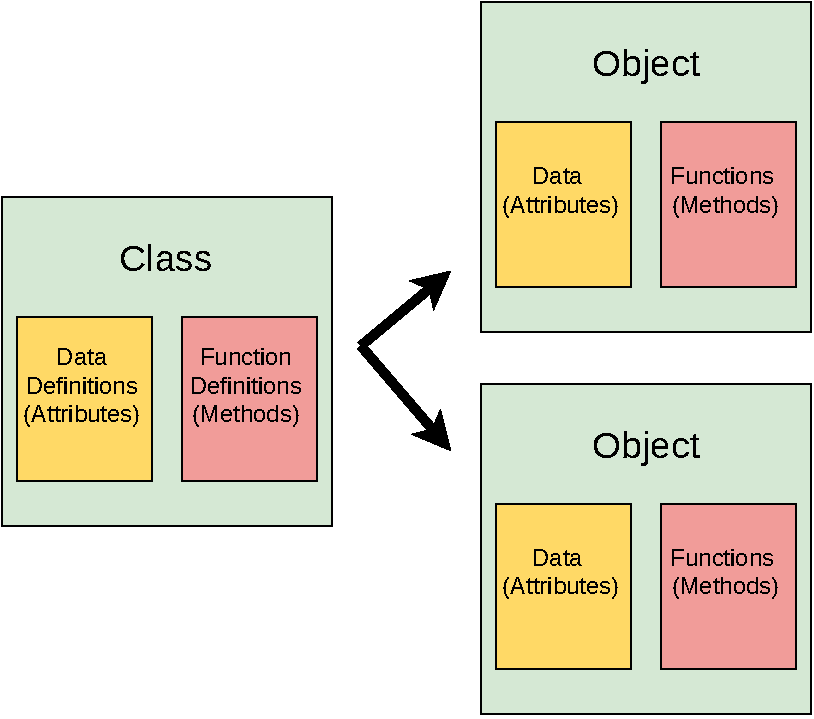
\includegraphics[width=1.0\textwidth]{Sources/class-object.pdf}
\end{adjustbox}
\end{center}
\end{frame}
\begin{frame}
\frametitle{Everything is an Object. Every Object has a Class}
\begin{itemize}
\item In Python, everything is an object except for variable names, which are references to objects
\vfill
\item Strings, floats, ints, lists, and tuples are types of objects. There are many more types of objects and users can define their own types of objects
\vfill
\item A class is a definition for a type of object. It defines how it is created, the data stored in it, and the functions attached to it
\vfill
\item We can write our own classes to create new types of objects to work with
\end{itemize}
\end{frame}
\begin{frame}
\frametitle{Many Objects to One Class}
\begin{itemize}
\item From a single class definition, an unlimited number of objects can be created
\vfill
\item Typically the class definition says it should accept some data to create the object
\vfill
\item Then when you have multiple objects of the same type (created from the same class), they will have the same functions (methods) attached to them, but different data stored within
\vfill
\item For example, we can create two different lists. They will have different contents, but we can
do
\texttt{.append}
on either of the lists
\end{itemize}
\end{frame}
\begin{frame}
\frametitle{Lists are Objects}
\begin{adjustbox}{width=0.425\textwidth, height=0.8\textheight, keepaspectratio}
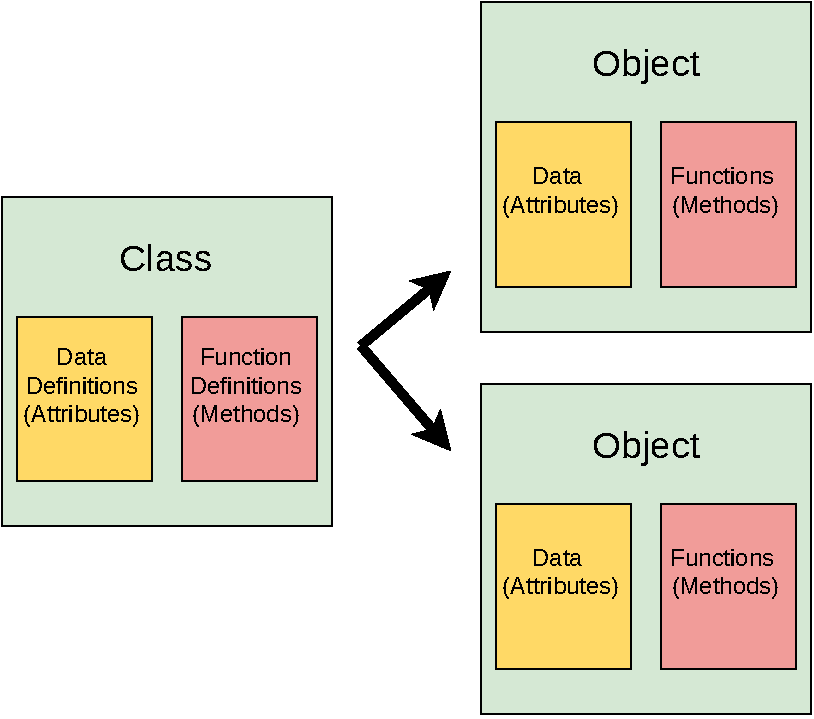
\includegraphics[width=1.0\textwidth]{Sources/class-object.pdf}
\end{adjustbox}
\hfill
\begin{adjustbox}{width=0.425\textwidth, height=0.8\textheight, keepaspectratio}
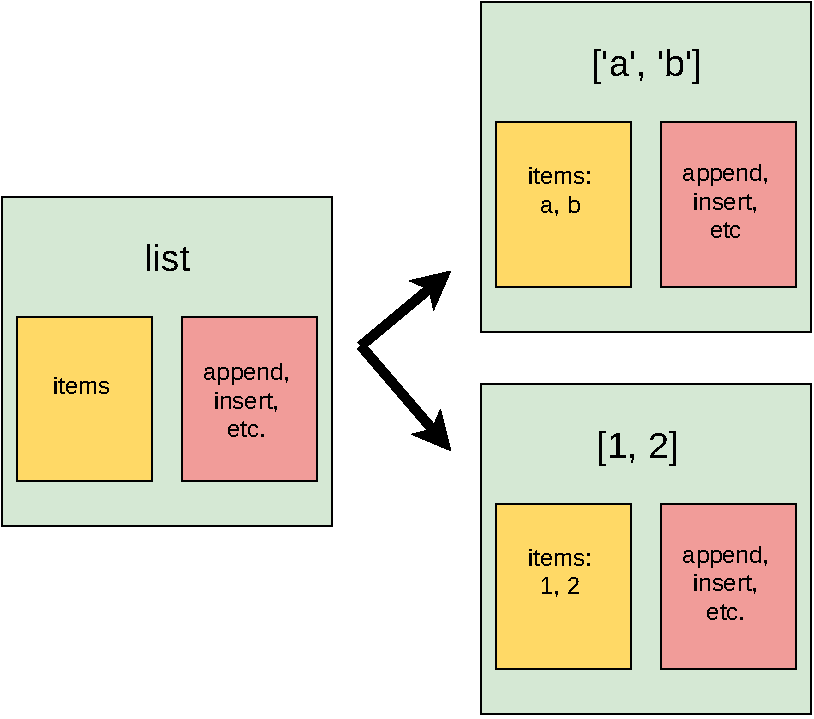
\includegraphics[width=1.0\textwidth]{Sources/list-object.pdf}
\end{adjustbox}
\end{frame}
\begin{frame}
\frametitle{We can Make Custom Objects Too}
\begin{adjustbox}{width=0.425\textwidth, height=0.8\textheight, keepaspectratio}
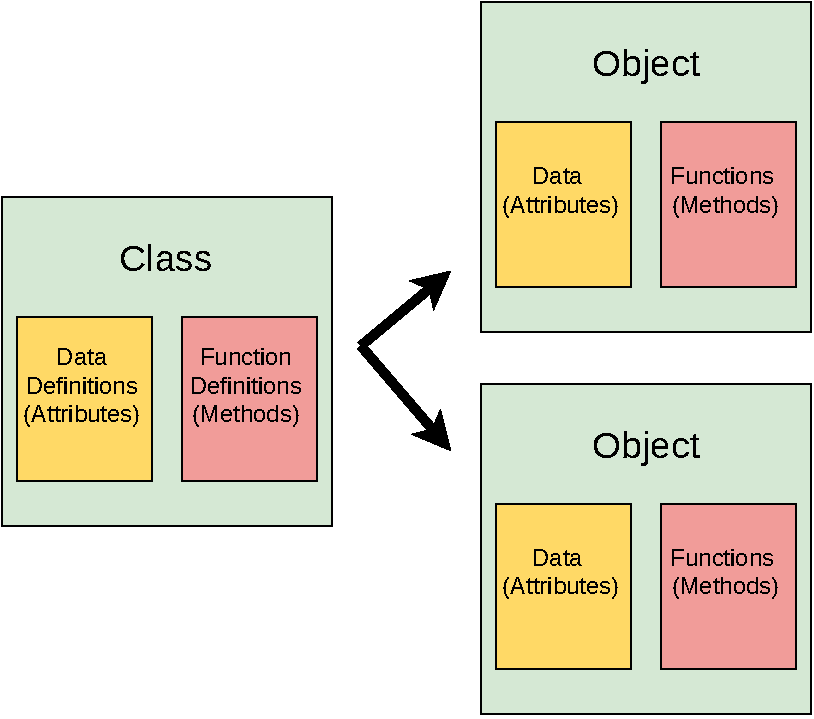
\includegraphics[width=1.0\textwidth]{Sources/class-object.pdf}
\end{adjustbox}
\hfill
\begin{adjustbox}{width=0.425\textwidth, height=0.8\textheight, keepaspectratio}
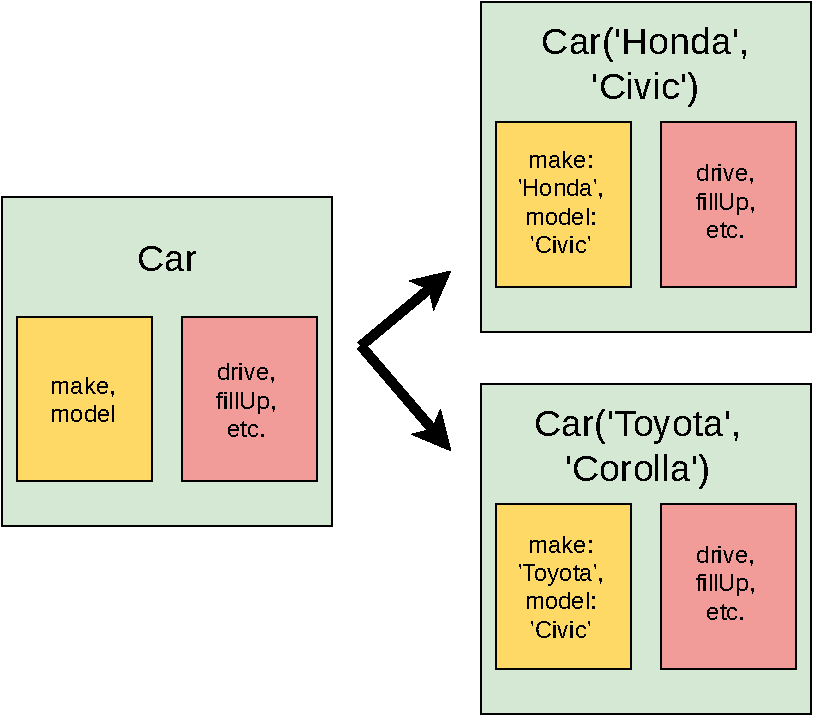
\includegraphics[width=1.0\textwidth]{Sources/car-object.pdf}
\end{adjustbox}
\end{frame}
\begin{frame}[fragile]
\frametitle{Creating and Using Objects}
\begin{itemize}
\item Constructing an object from a class looks like calling a function:
\end{itemize}
\begin{block}{Using Custom Classes in Python}
\small
\begin{minted}{python}

from car_example import Car

>>> my_car = Car('Honda', 'Civic')
>>> print(my_car)
Car(make='Honda', model='Civic')
>>> type(my_car)
car_example.Car
>>> my_car.make
'Honda'
>>> my_car.drive()
'The Honda Civic is driving away!'

\end{minted}
\end{block}
\end{frame}
\begin{frame}
\frametitle{Where we Will Focus in This Course}
\begin{itemize}
\item I will not be teaching you about creating general classes in this course. It is very useful but is generally more advanced. I encourage you to learn them outside the course.
\vfill
\item We covered this material for two reasons:
\vfill
\item To give a better understanding of how Python works in general, and why sometimes we call functions as
\texttt{something.my\_func()}
rather than
\texttt{my\_func()}
\vfill
\item We are going to use
\texttt{dataclasses}
to store our model data. They are
a simplified version of classes used mainly for storing data.
\end{itemize}
\end{frame}
\begin{frame}[fragile]
\frametitle{Dataclass Intro}
\begin{itemize}
\item An organized way to store our model input data:
\end{itemize}
\begin{block}{Using Dataclasses in Python}
\scriptsize
\begin{minted}{python}

from dataclasses import dataclass

@dataclass
class ModelInputs:
    interest_rates: tuple = (0.05, 0.06, 0.07)
    pmt: float = 1000

>>> inputs = ModelInputs(pmt=2000)
>>> print(inputs)
ModelInputs(interest_rates=(0.05, 0.06, 0.07), pmt=2000)
>>> type(inputs)
__main__.ModelInputs
>>> inputs.interest_rates
(0.05, 0.06, 0.07)
>>> inputs.pmt
2000

\end{minted}
\end{block}
\end{frame}
\begin{frame}
\frametitle{What, When and Why Dataclasses?}
\begin{itemize}
\item A
\texttt{dataclass}
is just a class which is more convenient to create, and
is typically used to group data together
\vfill
\item If you need to pass around multiple variables together, they make sense. For our models, we will want to pass around all the inputs, so one
\texttt{dataclass}
for all the
inputs to the model makes sense
\vfill
\item This way instead of having to pass around every input individually to every function, just pass all the input data as one argument
\vfill
\item Also enables easy tab-completion. What were the names of my inputs? Just hit tab after
\texttt{data.}
\end{itemize}
\end{frame}
\begin{frame}
\frametitle{Classes Example}
{
\setbeamercolor{block title}{bg=darkgreen}
\begin{block}{Working with Classes and Creating Dataclasses}
\begin{itemize}
\item We will keep working off of Python Basics.ipynb
\item For this example, also go and download car\_example.py and put it in the same folder
\item Now I will go through the example material under "Working with Classes"
\end{itemize}
\end{block}
}
\end{frame}
\begin{frame}
\frametitle{Python Classes Lab}
{
\setbeamercolor{block title}{bg=violet}
\begin{block}{Python Basics - Classes}
\begin{enumerate}
\item Keep working off of Python Basics Lab.ipynb
\item Make sure you have car\_example.py in the same folder
\item Please complete the exercises under "Working with Classes"
\end{enumerate}
\vfill
\begin{tabular*}{\textwidth}{@{\extracolsep{\fill}}ccc}
\toprule
\hfill & Resources: Slide \textcolor{blue}{\underline{\ref{labs:python-classes-lab-1-resources}}} & \hfill\\

\end{tabular*}
\end{block}
}
\label{labs:python-classes-lab-1}
\end{frame}
\end{section}
\begin{section}[Errors]{Error Handling}
\begin{frame}[fragile]
\frametitle{Python Error Handling}
\begin{itemize}
\item You have certainly already seen errors coming from your Python code. When they have come up, the code doesn't run.
\vfill
\item Sometimes you actually expect to get an error, and want to handle it in some way, rather than having your program fail.
\end{itemize}
\begin{block}<+>{Example}
\begin{minted}{python}

>>> my_list = ['a', 'b']
>>> try:
>>>     my_value = my_list[10]
>>> except IndexError:
>>>     print('caught the error')
caught the error

\end{minted}
\end{block}
\end{frame}
\begin{frame}
\frametitle{An Example where Error Handling is Useful}
\begin{itemize}
\item Let's say you're receiving annuities. There is a single annuity which produces \$100 for 5 years. You receive this annuity in year 0 and in year 3.
\vfill
\item You might define the annuity cash flows as a list of 100, 5 times (\texttt{[100] * 5})
\vfill
\item Then you want to come up with your overall cash flows, going out to 15 years
\end{itemize}
\end{frame}
\begin{frame}[fragile]
\frametitle{Applying Error Handling}
\begin{block}{Calculating the Sum of Unaligned Annuity Cash-Flows}
\small
\begin{minted}{python}

>>> annuity = [100] * 5
>>> annuities = [
>>>     annuity,
>>>     [0, 0, 0] + annuity
>>> ]
>>> n_years = 10
>>> output = [0] * n_years
>>> for i in range(n_years):
>>>     for ann in annuities:
>>>         try:
>>>             output[i] += ann[i]
>>>         except IndexError:
>>>             pass
>>> print(output)   
[100, 100, 100, 200, 200, 100, 100, 100, 0, 0]

\end{minted}
\end{block}
\end{frame}
\end{section}
\appendix
\newcounter{finalframe}
\setcounter{finalframe}{\value{framenumber}}
\begin{frame}
\frametitle{Lecture Resources}
{
\setbeamercolor{block title}{bg=teal}
\begin{block}{Lecture Resources}
\begin{enumerate}
\item \textcolor{blue}{\underline{\href{https://nickderobertis.github.io/fin-model-course/\_static/generated/pdfs/S4 Going Beyond an Initial Python Script.pdf}{Slides - Going Beyond an Initial Python Script}}}
\item \textcolor{blue}{\underline{\href{https://nickderobertis.github.io/fin-model-course/\_static/generated/pdfs/LN4 Going Beyond an Initial Python Script.pdf}{Lecture Notes - Going Beyond an Initial Python Script}}}
\item \textcolor{blue}{\underline{\href{https://nickderobertis.github.io/fin-model-course/\_static/Examples/Introduction/Python/Python Basics.ipynb}{Python Basics}}}
\item \textcolor{blue}{\underline{\href{https://nickderobertis.github.io/fin-model-course/\_static/Materials for Lab Exercises/Python Basics/Python Basics Lab.ipynb}{Python Basics Lab Exercises}}}
\item \textcolor{blue}{\underline{\href{https://docs.python.org/3/library/functions.html}{Python Built-in Functions Official Reference}}}
\item \textcolor{blue}{\underline{\href{http://cis.bentley.edu/sandbox/wp-content/uploads/Documentation-on-f-strings.pdf}{Guide to f-strings}}}
\item \textcolor{blue}{\underline{\href{https://nickderobertis.github.io/fin-model-course/\_static/Examples/Introduction/Python/car\_example.py}{Car Class Example}}}
\item \textcolor{blue}{\underline{\href{https://docs.python.org/3/reference/datamodel.html}{Python Classes Official Reference}}}
\item \textcolor{blue}{\underline{\href{https://docs.python.org/3/tutorial/errors.html}{Python Error Handling Official Reference}}}
\item \textcolor{blue}{\underline{\href{https://docs.python.org/3/library/exceptions.html}{Python Built-in Exceptions Official Reference}}}
\end{enumerate}
\vfill
\end{block}
}
\label{frames:resources}
\end{frame}
\begin{frame}
\frametitle{Python Conditionals Lab Resources}
{
\setbeamercolor{block title}{bg=teal}
\begin{block}{Python Basics - Conditionals Resources}
\begin{enumerate}
\item \textcolor{blue}{\underline{\href{https://nickderobertis.github.io/fin-model-course/\_static/Materials for Lab Exercises/Python Basics/Python Basics Lab.ipynb}{Python Basics Lab Exercises}}}
\item \textcolor{blue}{\underline{\href{https://nickderobertis.github.io/fin-model-course/\_static/generated/pdfs/S4 Going Beyond an Initial Python Script.pdf}{Slides - Going Beyond an Initial Python Script}}}
\end{enumerate}
\vfill
\begin{tabular*}{\textwidth}{@{\extracolsep{\fill}}ccc}
\toprule
\hfill & Exercise: Slide \textcolor{blue}{\underline{\ref{labs:python-conditionals-lab-1}}} & \hfill\\

\end{tabular*}
\end{block}
}
\label{labs:python-conditionals-lab-1-resources}
\end{frame}
\begin{frame}
\frametitle{Python Lists Lab Resources}
{
\setbeamercolor{block title}{bg=teal}
\begin{block}{Python Basics - Lists Resources}
\begin{enumerate}
\item \textcolor{blue}{\underline{\href{https://nickderobertis.github.io/fin-model-course/\_static/Materials for Lab Exercises/Python Basics/Python Basics Lab.ipynb}{Python Basics Lab Exercises}}}
\item \textcolor{blue}{\underline{\href{https://nickderobertis.github.io/fin-model-course/\_static/generated/pdfs/S4 Going Beyond an Initial Python Script.pdf}{Slides - Going Beyond an Initial Python Script}}}
\end{enumerate}
\vfill
\begin{tabular*}{\textwidth}{@{\extracolsep{\fill}}ccc}
\toprule
\hfill & Exercise: Slide \textcolor{blue}{\underline{\ref{labs:python-lists-lab-1}}} & \hfill\\

\end{tabular*}
\end{block}
}
\label{labs:python-lists-lab-1-resources}
\end{frame}
\begin{frame}
\frametitle{Python Functions Lab Resources}
{
\setbeamercolor{block title}{bg=teal}
\begin{block}{Python Basics - Functions Resources}
\begin{enumerate}
\item \textcolor{blue}{\underline{\href{https://nickderobertis.github.io/fin-model-course/\_static/Materials for Lab Exercises/Python Basics/Python Basics Lab.ipynb}{Python Basics Lab Exercises}}}
\item \textcolor{blue}{\underline{\href{https://nickderobertis.github.io/fin-model-course/\_static/generated/pdfs/S4 Going Beyond an Initial Python Script.pdf}{Slides - Going Beyond an Initial Python Script}}}
\end{enumerate}
\vfill
\begin{tabular*}{\textwidth}{@{\extracolsep{\fill}}ccc}
\toprule
\hfill & Exercise: Slide \textcolor{blue}{\underline{\ref{labs:python-functions-lab-1}}} & \hfill\\

\end{tabular*}
\end{block}
}
\label{labs:python-functions-lab-1-resources}
\end{frame}
\begin{frame}
\frametitle{Python Data Types Lab Resources}
{
\setbeamercolor{block title}{bg=teal}
\begin{block}{Python Basics - Data Types Resources}
\begin{enumerate}
\item \textcolor{blue}{\underline{\href{https://nickderobertis.github.io/fin-model-course/\_static/Materials for Lab Exercises/Python Basics/Python Basics Lab.ipynb}{Python Basics Lab Exercises}}}
\item \textcolor{blue}{\underline{\href{https://nickderobertis.github.io/fin-model-course/\_static/generated/pdfs/S4 Going Beyond an Initial Python Script.pdf}{Slides - Going Beyond an Initial Python Script}}}
\end{enumerate}
\vfill
\begin{tabular*}{\textwidth}{@{\extracolsep{\fill}}ccc}
\toprule
\hfill & Exercise: Slide \textcolor{blue}{\underline{\ref{labs:python-data-types-lab-1}}} & \hfill\\

\end{tabular*}
\end{block}
}
\label{labs:python-data-types-lab-1-resources}
\end{frame}
\begin{frame}
\frametitle{Python Classes Lab Resources}
{
\setbeamercolor{block title}{bg=teal}
\begin{block}{Python Basics - Classes Resources}
\begin{enumerate}
\item \textcolor{blue}{\underline{\href{https://nickderobertis.github.io/fin-model-course/\_static/Materials for Lab Exercises/Python Basics/Python Basics Lab.ipynb}{Python Basics Lab Exercises}}}
\item \textcolor{blue}{\underline{\href{https://nickderobertis.github.io/fin-model-course/\_static/generated/pdfs/S4 Going Beyond an Initial Python Script.pdf}{Slides - Going Beyond an Initial Python Script}}}
\item \textcolor{blue}{\underline{\href{https://nickderobertis.github.io/fin-model-course/\_static/Examples/Introduction/Python/car\_example.py}{Car Class Example}}}
\end{enumerate}
\vfill
\begin{tabular*}{\textwidth}{@{\extracolsep{\fill}}ccc}
\toprule
\hfill & Exercise: Slide \textcolor{blue}{\underline{\ref{labs:python-classes-lab-1}}} & \hfill\\

\end{tabular*}
\end{block}
}
\label{labs:python-classes-lab-1-resources}
\end{frame}
\setcounter{framenumber}{\value{finalframe}}
\end{document}